%-------------------------------------------------
%	Version: 0.0
%	fecha de entrega 5 febrero 2021
%
%-------------------------------------------------

\documentclass[11pt]{report}

%packages
\usepackage{graphicx}
\usepackage{subcaption}

\usepackage[utf8]{inputenc}
\usepackage[spanish, es-nodecimaldot]{babel}
\usepackage{setspace}
\usepackage{ragged2e}

\usepackage{amsmath}
\usepackage{amsthm}
\usepackage{amssymb}
\usepackage{mathtools}
\usepackage{siunitx}
\usepackage[thinc]{esdiff} %derivadas faciles
\usepackage{physics} %algunos simbolos de derivadas

%path donde se encuentran las imagenes
\graphicspath{ {./figuras/} }

%---------------------------------------------------------------
%ABREVIACIONES DE COMANDOS
%---------------------------------------------------------------

\theoremstyle{plain}
\newtheorem{thm}{Teorema}[chapter] % reset theorem numbering for each chapter

\theoremstyle{definition}
\newtheorem{defn}[thm]{Definición} % definition numbers are dependent on theorem numbers
\newtheorem{exmp}[thm]{Ejemplo} % same for example numbers

\newcommand{\chaptercontent}{
\section{Basics}
\begin{defn}Here is a new definition.\end{defn}
\begin{thm}Here is a new theorem.\end{thm}
\begin{thm}Here is a new theorem.\end{thm}
\begin{exmp}Here is a good example.\end{exmp}
\subsection{Some tips}
\begin{defn}Here is a new definition.\end{defn}
\section{Advanced stuff}
\begin{defn}Here is a new definition.\end{defn}
\subsection{Warnings}
\begin{defn}Here is a new definition.\end{defn}
}

\usepackage{biblatex}
%\addbibresource{Tarea1.bib}

\begin{document}

\begin{titlepage}
\title{Titulo_del_trabajo}

%-------------------------------------------------
%PORTADA
%-------------------------------------------------

	\centering
	{\scshape\LARGE Universidad Autónoma de Yucatán  \\ Facultad de ingeniería\par}
	\vspace{1cm}
	{\scshape\Large Métodos matemáticos de la física\par}
	\vspace{1.5cm}
	{\huge\bfseries Segundo examen\par}
	\vspace{0.7cm}
	{\begin{figure}[!h]
	\centering
    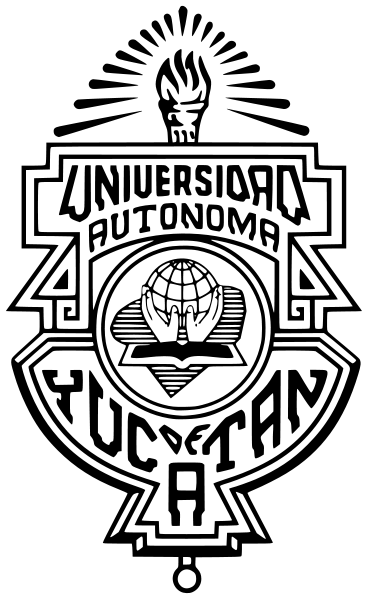
\includegraphics[scale=0.3]{UADY.png}
	\end{figure}}
	\vspace{0.7cm}
	{\Large\itshape Erick Al. Casanova Cortés\par}
	{\Large\itshape Matricula: 15014866\par}
	\vfill
	{\scshape\Large Docente\par
	Dr. Miguel Zambrano\par}
	\vfill
	{\Large{\bfseries Fecha de entrega: 5 Febrero 2021} }

	\vfill
	
\end{titlepage}

%-------------------------------------------------
%Inicio del documento
%-------------------------------------------------

%-------------------------------------------------
%Primer Ejercicio
%-------------------------------------------------
\textit{Una esfera hueca de radio que esta dividida en dos por el ecuador por un aislante delgado. La mitad superior se encuentra a un potencial constante $V_0$ y el hemisferio inferior a un potencial nulo, como se muestra en la figura.}\\

\textit{Demostrar que el potencial dentro de la esfera esta dado por:}

\begin{equation}
	\label{eq:final_in}
	\phi(r, \theta) = \frac{V_0}{2}\{ 1 +\sum^\infty_{n=0}(-1)^n \frac{(2n)!(4n+3)}{2^{2n}(n!)(2n+2)}\left(\frac{r}{c}\right)^{2n+1}P_{2n+1}\cos(\theta)\}
\end{equation}

\textit{mientras que en el potencial exterior es:}
\begin{equation}
	\label{eq:final_out}
	\phi(r, \theta) = \frac{V_0c}{2r}\{ 1 +\sum^\infty_{n=0}(-1)^n \frac{(2n)!(4n+3)}{2^{2n}(n!)(2n+2)}\left(\frac{c}{r}\right)^{2n+1}P_{2n+1}\cos(\theta)\}
\end{equation}


\textit{Ayuda: resolver la ecuación de Laplace $\nabla^2 \phi(r,\theta,\varphi) =0$ en coordenadas esféricas}\\


%--- resolución de la ecuación de Laplace

Primero haremos el cálculo de la ecuación de Laplace en coordenadas esféricas, la cual está expresada de la forma

\begin{equation} %eq laplace en coordenadas esfericas
\label{eqn:laplace_spherical_coordinates}
	\left(\frac{1}{r^2}\pdv{r}r^2\pdv{r} + \frac{1}{r^2\sin\theta}\pdv{\theta}\sin\theta\pdv{\theta} + \frac{1}{r^2\sin^2\theta}\pdv[2]{\varphi}\right)F(r,\theta,\varphi) = 0
\end{equation}


De esto partimos que la función $F(r,\theta,\varphi)$ puede expresarse de tal forma que $F(r,\theta,\varphi)=R(r)\Theta(\theta)\Phi(\varphi)$. Por lo que podemos multiplicar ambas partes de la ecuación \ref{eqn:laplace_spherical_coordinates} por $\frac{r^2}{F}$, lo cual queda expresado como:

\begin{equation*} %multiplicando por r^2/f
	\frac{r^2}{F} \left(\frac{1}{r^2}\pdv{r}r^2\pdv{r} + \frac{1}{r^2\sin\theta}\pdv{\theta}\sin\theta\pdv{\theta} + \frac{1}{r^2\sin^2\theta}\pdv[2]{\varphi}\right)F(r,\theta,\varphi) = 0
\end{equation*}

Sustituyendo a $F(r,\theta,\varphi)$ por la propuesta


\begin{equation*} %sustituir por funciones dep
	\frac{r^2}{R\Theta\Phi} \left(\frac{1}{r^2}\pdv{r}r^2\pdv{r} + \frac{1}{r^2\sin\theta}\pdv{\theta}\sin\theta\pdv{\theta} + \frac{1}{r^2\sin^2\theta}\pdv[2]{\varphi}\right)R\Theta\Phi= 0
\end{equation*}

Ahora se expandirá la ecuación a conveniencia de tal modo que dejaremos los términos que dependen del radio de un lado y agruparemos los términos que dependen del ángulo polar o azimutal; quedando entonces:


\begin{equation*}%agrupar terminos
	\frac{1}{R}\pdv{r}r^2\pdv{r}R = -\frac{1}{\Theta\Phi}\left(\frac{1}{\sin\theta}\pdv{\theta}\sin\theta\pdv{\theta} + \frac{1}{\sin^2\theta}\pdv[2]{\varphi}\right)\Theta\Phi
\end{equation*}

Como $r$, $\theta$ y $\varphi$ son variables independientes quiere decir que ambos términos son iguales a una constante, lo que quiere decir que

\begin{equation}
\label{eqn:r_dep_sol_laplace} %parte de r
	\frac{1}{R}\pdv{r}r^2\pdv{r}R = \mathcal{C}
\end{equation}

\begin{equation}
\label{eqn:theta_phi_dep_sol_laplace} %parte de teta y phi
	-\frac{1}{\Theta\Phi}\left(\frac{1}{\sin\theta}\pdv{\theta}\sin\theta\pdv{\theta} + \frac{1}{\sin^2\theta}\pdv[2]{\varphi}\right)\Theta\Phi = \mathcal{C}
\end{equation}


si a la ecuación \ref{eqn:theta_phi_dep_sol_laplace} la multiplicamos por $\sin^2\theta$ tenemos:

\begin{equation*} % sin^2 tta
	-\frac{1}{\Theta\Phi}\left(\sin\theta\pdv{\theta}\sin\theta\pdv{\theta} + \pdv[2]{\varphi}\right)\Theta\Phi = \mathcal{C}\sin^2\theta
\end{equation*}

Agrupando la ecuación en sus términos dependientes nos queda la siguiente igualdad:

\begin{equation*} %agrupar
	\frac{1}{\Theta}\sin\theta\pdv{\theta}\sin\theta	\pdv{\theta}\Theta+\mathcal{C}\sin^2\theta = - \frac{1}{\Phi}\pdv[2]{\varphi}\Phi 
\end{equation*}

Como anteriormente se vio, para que esta igualdad se cumpla, ambas partes de dicha ecuación deberán ser igualadas a una constante. Lo cual queda de la siguiente forma:

\begin{equation}
	\label{eq:teta_sol}
	\frac{1}{\Theta}\sin\theta\pdv{\theta}\sin\theta	\pdv{\theta}\Theta+\mathcal{C}\sin^2\theta = \mathcal{B}
\end{equation}

\begin{equation}
	\label{eq:phi_sol}
	- \frac{1}{\Phi}\pdv[2]{\varphi}\Phi = \mathcal{B}
\end{equation}

Haciendo un despeje de la ecuación \ref{eq:phi_sol} podemos ver que podemos encontrar una solución, como se ve a continuación

\begin{equation*}
	\pdv[2]{\varphi}\Phi = -\Phi\mathcal{B}
\end{equation*}

al resolver la ecuación diferencial podemos ver que $\Phi$ está dada por:

\begin{equation*}
	\Phi(\varphi) = e^{\pm i\sqrt{\mathcal{B}}\varphi}
\end{equation*}

Si hacemos un análisis de esta ecuación podemos ver que es periódica con un ciclo de $2\pi$, lo que implica:

\begin{equation*}
	e^{\pm i\sqrt{\mathcal{B}}\varphi} = e^{\pm i\sqrt{\mathcal{B}}(\varphi+2\pi)}
\end{equation*}

En otras palabras, lo que quiere decir es que $\sqrt{\mathcal{B}}$ debe ser un entero, y por fines prácticos haremos la igualdad $\sqrt{\mathcal{B}} = k^2$, regresando a la solución tenemos entonces que la parte de $\Phi$ queda expresada como:

\begin{equation*}
	\Phi(\varphi) = e^{\pm ik^2\varphi}
\end{equation*}

%-- teta

Pasando ahora a la parte que depende de $\Theta$, partimos de la ecuación \ref{eq:teta_sol} y tomando la igualdad que encontramos anterior, la cual nos afirma que $\sqrt{\mathcal{B}} = k^2$

\begin{equation*}
	\frac{1}{\Theta}\sin\theta\pdv{\theta}\sin\theta	\pdv{\theta}\Theta+\mathcal{C}\sin^2\theta = k^2
\end{equation*}

Para hacer resolver esta ecuación diferencial tendremos que hacer un cambio de variable, el cual será proponer una función a modo que:

\begin{equation*}
	x=\cos\theta
\end{equation*}

Haciendo la regla de la cadena podemos ver:

\begin{align*}
	\pdv{\theta} &= \pdv{x}{\theta}\pdv{x}\\
	&=-\sin\theta \pdv{x}
\end{align*}

Por otra parte tenemos la igualdad

\begin{equation*}
	\sin^2\theta = 1-\cos^2\theta
\end{equation*}

Por lo que con nuestro cambio de variable podemos ver que $\sin^2\theta = 1-x^2$. Sustituyendo en la ecuación y haciendo $\Theta(\theta) = y(x)$ podemos ver que:

\begin{equation*}
	\dv{x}\left(1-x^2\right)\dv{x}y+\left(\mathcal{C}-\frac{k^2}{1-x^2}\right)y=0
\end{equation*}

Con esta ecuación podemos ver el conflicto de que diverge para $x=\pm 1$, a menos que hagamos que $\mathcal{C} = c(c+1)$ lo que nos lleva a

\begin{equation*}
	\dv{x}\left(1-x^2\right)\dv{x}y+\left(c(c+1)-\frac{k^2}{1-x^2}\right)y=0
\end{equation*}

Otra cosa que tenemos que tener en cuenta es que para obtener una solución aceptable debemos hacer que $-c\leq k \leq c$. Entonces la solución de esta ecuación se puede expresar como su polinomio de Legendre asociado:

\begin{equation*}
	y(x)=P_c^{|k|}(x)
\end{equation*}

La solución para $k=0$
\begin{equation*}
	\dv{x}\left(1-x^2\right)\dv{x}y(x)+c(c+1)y(x)=0
\end{equation*}

Regresando entonces a nuestras variables iniciales

\begin{equation*}
	\Theta(\theta)=P_c^{|k|}(\cos\theta)
\end{equation*}

%--radio

La parte que depende del radio de la ecuación de Laplace lo vimos anteriormente, y con las condiciones que hemos generado hasta ahora podemos expresarla de tal modo que:

\begin{equation*}
	r^2\dv[2]{r}R+2r\dv{r}R=c(c+1)R
\end{equation*}

Esta parte se debe resolver con un cambio de variable especial, se hará

\begin{align*}
	r&=e^t,\\
	t&=\ln{r},\\
	\dv{t}{r}&=\frac{1}{r}
\end{align*}

Entonces nos queda la siguiente expresión:
\begin{equation*}
	r^2\dv[2]{R}{r}+2r\dv{R}{r}=\dv[2]{R}{t}+\dv{R}{t}
\end{equation*}

la cual se expresa como:
\begin{equation*}
	\dv[2]{R}{t}+\dv{R}{t}=c(c+1)R
\end{equation*}

Esta ecuación diferencial se resuelve de manera sencilla, la cual podemos ver que la solución se representa como:

\begin{equation*}
	R(t)=e^{kt}
\end{equation*}

Entonces

\begin{align*}
	\dv{R}{t}&=ke^{kt}\\
	\dv[2]{R}{t}&=k^2e^{kt}
\end{align*}

y $k$ puede ser determinada por:

\begin{equation*}
	k^2+k=c(c+1)
\end{equation*}

Entonces es evidente que

\begin{equation*}
	k=
	\begin{cases}
		c,\\
		-c-1
	\end{cases}
\end{equation*}

Entonces:

\begin{equation*}
	R(t)=
	\begin{cases}
		e^{ct}=e^{c\ln{r}}=r^c\\
		e^{-(c+1)t}=e^{-(c+1)\ln{r}}=\frac{1}{r^{c+1}}
	\end{cases}
\end{equation*}

Entonces la solución general de la ecuación de Laplace está dada por:

\begin{equation}
	\label{eq:sol_laplace}
	F(r,\theta)=\sum^\infty_{c=0}\left(a_c r^c + b_c \frac{1}{r^{c+1}}\right)P_c(\cos\theta)
\end{equation}

Los coeficientes $a$ y $b$ son determinados por las condiciones de frontera

%- ahora si el ejercicio

Partiendo de la solución anterior (eq: \ref{eq:sol_laplace}), ahora la función será el potencial que satisface dicha ecuación, tenemos que conocer los coeficientes por las condiciones de frontera, por lo que analizando dichas condiciones vemos que:
\begin{equation*}
	V=
	\begin{cases}
		V_o \text{ para } 0\leq\theta\leq\pi/2\\
		0 \text{ para } \pi/2\leq\theta\leq\pi
	\end{cases}
\end{equation*}

Siendo las condiciones tales que: $b=0$ y $r=r'$ tenemos entonces:

\begin{equation*}
	\sum^\infty_{c=0} a_c r'^c P_c(\cos\theta) = V
\end{equation*}



\begin{equation*}
	\sum^\infty_{c=0} a_c r'^c \int^\pi_0  P_c(\cos\theta) P_n(\cos\theta)\sin\theta \dd{\theta} = \int^\pi_0 VP_n(\cos\theta)\sin\theta\dd{\theta}
\end{equation*}

Como:

\begin{equation*}
	\int^\pi_0  P_c(\cos\theta) P_n(\cos\theta)\sin\theta \dd{\theta} = \int^1_{-1}P_l(x)P_n(x)\dd{x}=\frac{2}{2n+1}\delta_{nl}
\end{equation*}

\begin{equation*}
	a_nc^n\frac{2}{2n+1}=\int^\pi_0 VP_n(\cos\theta)\sin\theta\dd{\theta}
\end{equation*}

Cambiando $n$ a $l$ y $\cos\theta$ a $x$

\begin{equation*}
	a_l = \frac{2l+1}{2c^l}V_o\int^1_0P_l(x)\dd{x}
\end{equation*}

\begin{equation*}
	v=\sum^\infty_{c=0} \frac{2l+1}{2c^l}V_o\int^1_0P_l(x)\dd{x} \frac{r^l}{c^l} P_l(\cos\theta)
\end{equation*}

podemos ver que:

\begin{align*}
	a_0 &= \frac{1}{2}V_0\\
	a_1 &= \frac{3}{4c}V_0\\
	a_2 &= 0\\
	a_3 &= -\frac{7}{16c^3}V_0\\
\end{align*}

\begin{align*}
	\int^1_0 P_l(x)\dd{x} = \frac{1}{2l+l}(P_{l-1}(0)-P_{l+1}(0))
\end{align*}

entonces $P_{l-1}(0)=P_{l+1}(0)=0$, esto implica que $a_l = 0$ para $\forall l \neq a_0$, entonces:

\begin{equation*}
	V = \frac{1}{2}V_0 + \sum^\infty_{c=0} a_{2n+1}r^{2n+1}P_{2n+1}(\cos\theta)
\end{equation*}

de modo que

\begin{align*}
	a_{2n+1}=\frac{4n+3}{2c^{2n+1}}V_0\int^1_0P_{2n+1}(x)\dd{x}
\end{align*}

Como 

\begin{align*}
	\int^1_0 P_{2n+1}(x)\dd{x} = \frac{P_{2n}(0)-P_{2n+2}(0)}{4n+3}
\end{align*}


igual se sabe que:

\begin{align*}
	P_{2n}(0) = (-1)^n\frac{(2n)!}{2^{2n}(n!)^2}
\end{align*}

Entonces

\begin{align*}
	\int^1_0P_{2n+1}(x)\dd{x} = \frac{1}{4n+3} (-1)^n\frac{(2n)!}{2^{2n}(n!)^2}\frac{4n+3}{2n+2} 
\end{align*}

Entonces V dentro de la estefa esta dado por

\begin{align*}
	V = \frac{V_0}{2}\{ 1 +\sum^\infty_{n=0}(-1)^n \frac{(2n)!(4n+3)}{2^{2n}(n!)(2n+2)}\left(\frac{r}{c}\right)^{2n+1}P_{2n+1}\cos(\theta)\}
\end{align*}

La cual es igual a la ecuación \ref{eq:final_in}, por lo que la primera parte se cumple, ahora para fuera de la esfera requerimos que $r\rightarrow\infty$, entonces los términos $a_l$ deben ser cero, quedando enterminos de $b_l$

\begin{equation*}
	\sum^\infty_{l=0}b_l\frac{1}{c^{l+1}}P_l(\cos\theta)=V
\end{equation*}

Y degido del argumento anterior

\begin{equation*}
	b_l\frac{1}{c^{l+1}}=\frac{2l+1}{2}V_0\int^1_0P_l(x)\dd{x}
\end{equation*}

lo que nos queda entonces:

\begin{equation*}
	V = \frac{V_0c}{2r}\{ 1 +\sum^\infty_{n=0}(-1)^n \frac{(2n)!(4n+3)}{2^{2n}(n!)(2n+2)}\left(\frac{c}{r}\right)^{2n+1}P_{2n+1}\cos(\theta)\}
\end{equation*}

Lo que también resulta igual a la ecuación \ref{eq:final_out}, por lo que ambas partes quedan demostradas
%-------------------------------------------------
%Final del documento
%-------------------------------------------------

\end{document}
